\section{Ôn tập chương 1 - Hàm số lượng giác và phương trình lượng giác}
\caulc
\Opensolutionfile{ans}[ans/1-OTC1]
%%%==============EX_1============%%%
\begin{ex}%[1D1N1-2]
	Góc có số đo $130^\circ$ đổi sang rađian là
	\choice
	{\True $\dfrac{13\pi}{18}$}
	{$\dfrac{13}{18}$}
	{$\dfrac{18\pi}{13}$}
	{$\dfrac{18}{13}$}
	\loigiai{
		Áp dụng công thức $\alpha^\circ=\dfrac{\alpha \pi}{180} rad$ ta được $130^\circ=\dfrac{13\pi}{18}$.
	}
\end{ex}
%%%============EX_2==============%%%
\begin{ex}%[1D1N1-3]
	\immini[thm]{
	Cho lục giác đều $ABCDEF$ nội tiếp đường tròn lượng giác có gốc là $A$ (như hình vẽ bên). Số đo tổng quát của góc lượng giác $\left(OA,OF\right)$ bằng
	\choice[1]
	{$-60^\circ$}
	{$300^\circ$}
	{$-60^\circ$ hoặc $300^\circ$}
	{\True $-60^\circ+k360^\circ, k\in {\bf \mathbb{Z}}$}	
	}
	{
	\begin{tikzpicture}[scale=1, font=\footnotesize, line join=round, line cap=round,>=stealth]
		\def \R{2} \def\rt{.03}
		\def\xmin{-2.5} \def\xmax{3}
		\def\ymin{-2.5} \def\ymax{3}
		%\draw[color=gray!50,dashed] (\xmin,\ymin) grid (\xmax,\ymax);
		\path 
		(0,0) coordinate (O)
		(0:\R) coordinate (A)
		(60:\R) coordinate (B)
		(120:\R) coordinate (C)
		(180:\R) coordinate (D)
		(240:\R) coordinate (E)
		(300:\R) coordinate (F)
		;
		\draw[->] (\xmin,0)--(0,0) node[below left]{$O$} --(\xmax,0) node[below left] {$x$};
		\draw[->] (0,\ymin)--(0,\ymax) node[below right] {$y$};
		\draw[fill=black] (0,0) circle (\rt);
		\draw[blue] (O) circle (\R) ;
		\draw pic[draw,stealth-,angle radius=3mm,red]{angle=F--O--A};
		\draw[red,thick] (A)--(O)--(F) ;
		\draw (A)--(B)--(C)--(D)--(E)--(F)--cycle;
		\foreach \p/\g in {A/-45,B/90,C/90,D/220,E/-90,F/-90} \fill[black] (\p) circle(1pt)+(\g:0.3) node{$\p$};   
	\end{tikzpicture}		
	}
	
	\loigiai{}
\end{ex}
%%%============EX_3==============%%%
\begin{ex}%[1D1N4-1]
	Cho đồ thị hàm số $y=\cos x$ trên đoạn $\left[-\pi;2\pi \right]$, giá trị của $x$ để hàm số $y=\cos x$ nhận giá trị bằng 1 là
	\begin{center}
	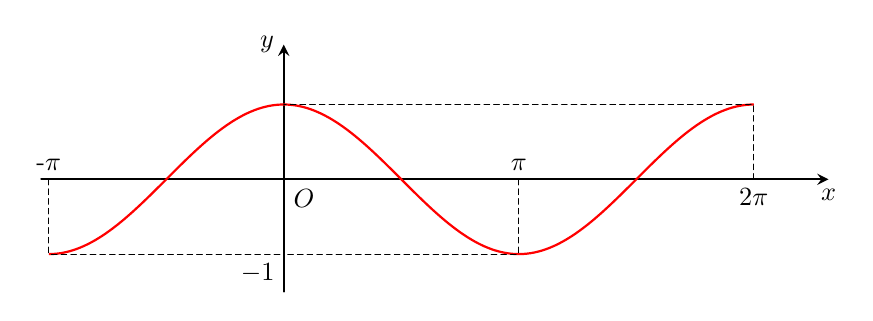
\begin{tikzpicture}[line join=round, line cap=round,thick,>=stealth,scale=.95,transform shape]
	\tikzset{every node/.style={font=\normalsize}}
				 	\pgfmathsetmacro{\xmin}{-pi}
				 	\pgfmathsetmacro{\xmax}{2*pi}
				 	\def\ymin{-1.5} \def\ymax{1.5} \def\rt{.03}
				 	\draw[->](\xmin-.1,0)--(\xmax+1,0) node[below]{$x$};
				 	\draw[->](0,-1.5)--(0,1.8) node[left]{$y$};
				 	\draw (0,0) node[below right]{$O$};
		\begin{scope} 
			\clip (\xmin,\ymin) rectangle (\xmax,\ymax);
				\draw[domain=\xmin:\xmax,samples=200,smooth,red] plot(\x,{cos(\x r)});
			\end{scope}
			\draw[dash pattern=on 2pt off 1.5pt,thin] 
			(-pi,0)node[above]{-$\pi$}|-(0,-1)node[below left]{$-1$}
			(2*pi,0)node[below]{$2\pi$}|-(0,1) 
			(pi,0)node[above]{$\pi$}|-(0,-1)	;
				 \end{tikzpicture}		
	\end{center}
	\choice
	{$x=-\pi$}
	{$x=\pi$}
	{\True $x=0$}
	{$x=\dfrac{\pi}{2}$}
	\loigiai{}
\end{ex}
%%%============EX_4==============%%%
\begin{ex}%[1D1N4-3]
	Hàm số $y=\tan x$ đồng biến trên khoảng
	\choice
	{$\left(-\pi;0\right)$}
	{$\left(0;\pi \right)$}
	{\True $\left(\dfrac{\pi}{2};\pi \right)$}
	{$\left(0;5\right)$}
	\loigiai{
	Tập xác định $\mathscr{D}=\mathbb{R}\setminus \left\{\dfrac{\pi}{2}\right\}$.\\
	Hàm số $y=\tan x$ đồng biến trên từng khoảng xác định nên nó đồng biến trên khoảng $\left(\dfrac{\pi}{2};\pi \right)$.}
\end{ex}
%%%============EX_5==============%%%
\begin{ex}%[1D1N4-4]
	Khẳng định nào dưới đây là đúng?
	\choice
	{Hàm số $y=\cos x$ là hàm số lẻ}
	{Hàm số $y=\cot x$ là hàm số chẵn}
	{\True Hàm số $y=\sin x$ là hàm số lẻ}
	{Hàm số $y=\tan x$ là hàm số chẵn}
	\loigiai{
Các hàm số $y=\sin x$, $y=\tan x$, $y=\cot x$ là hàm số lẻ.\\
Hàm số $y=\cos x$ là hàm số chẵn.
}
\end{ex}
%%%============EX_6==============%%%
\begin{ex}%[1D1H5-3]
	Tất cả các nghiệm của phương trình $\sin 2x=\dfrac{\sqrt{2}}{2}$ là
	\choice
	{$\hoac{&x=\dfrac{\pi}{4}+k2\pi\\&x=\dfrac{3\pi}{4}+k2\pi} \left(k\in \mathbb{Z}\right)$}
	{$\hoac{&x=\dfrac{\pi}{4}+k\pi\\&x=\dfrac{3\pi}{4}+k\pi} \left(k\in \mathbb{Z}\right)$}
	{\True $\hoac{&x=\dfrac{\pi}{8}+k\pi\\&x=\dfrac{3\pi}{8}+k\pi} \left(k\in \mathbb{Z}\right)$}
	{$\hoac{&x=\dfrac{\pi}{8}+k2\pi\\&x=\dfrac{3\pi}{8}+k2\pi} \left(k\in \mathbb{Z}\right)$}
	\loigiai{
Ta có
\allowdisplaybreaks
\begin{eqnarray*}
	&&\sin 2x=\dfrac{\sqrt{2}}{2}\\
	&\Leftrightarrow&\sin 2x=\sin\dfrac{\pi}{4}\\
	&\Leftrightarrow&\hoac{&2x=\dfrac{\pi}{4}+k2\pi\\&2x=\pi-\dfrac{\pi}{4}+k2\pi}\\
	&\Leftrightarrow&\hoac{&x=\dfrac{\pi}{8}+k\pi\\&x=\dfrac{3\pi}{8}+k\pi} \left(k\in \mathbb{Z}\right).
\end{eqnarray*}	
}
\end{ex}
%%%============EX_7==============%%%
\begin{ex}%[1D1H5-5]
	Tất cả các nghiệm của phương trình $\sin 2x-\cos x=0$ là
	\choice
	{\True $x=\dfrac{\pi}{2}+k\pi;x=\dfrac{\pi}{6}+k2\pi;x=\dfrac{5\pi}{6}+k2\pi;k\in \mathbb{Z}$}
	{$x=\dfrac{-\pi}{6}+k\dfrac{2\pi}{3};\dfrac{\pi}{2}+k2\pi;x=\dfrac{5\pi}{6}+k2\pi;k\in \mathbb{Z}$}
	{$x=\dfrac{\pi}{6}+k\dfrac{2\pi}{3};\dfrac{-\pi}{2}+k2\pi;x=\dfrac{5\pi}{6}+k2\pi;k\in \mathbb{Z}$}
	{$x=\dfrac{-\pi}{6}+k\dfrac{2\pi}{3};\dfrac{-\pi}{2}+k2\pi;x=\dfrac{5\pi}{6}+k2\pi;k\in \mathbb{Z}$}
	\loigiai{
Ta có
\allowdisplaybreaks
\begin{eqnarray*}
	&&\sin 2x-\cos x=0\\
	&\Leftrightarrow&\sin 2x=\cos x\\
	&\Leftrightarrow&\sin 2x=\sin\left(\dfrac{\pi}{2}-x\right)\\
	&\Leftrightarrow&\hoac{&2x=\dfrac{\pi}{2}-x+k2\pi\\&2x=\pi -\dfrac{\pi}{2}+x+k2\pi}\\
	&\Leftrightarrow&\hoac{&x=\dfrac{\pi}{6}+k\dfrac{2\pi}{3}\\&x=\dfrac{\pi}{2}+k2\pi}\\
	&\Leftrightarrow&\hoac{&x=\dfrac{\pi}{2}+k\pi\\&x=\dfrac{\pi}{6}+k2\pi\\&x=\dfrac{5\pi}{6}+k2\pi},k\in \mathbb{Z}.
\end{eqnarray*}	
}
\end{ex}
%%%============EX_8==============%%%
\begin{ex}%[1D1H4-7]
	Dùng đồ thị hàm số $y=\sin x$ (tham khảo hình vẽ) để xác định số nghiệm của phương trình $2\sin x-1=0$ trên khoảng $\left(-\dfrac{\pi}{2};2\pi \right)$.
	\begin{center}
	\begin{tikzpicture}[line join=round, line cap=round,thick,>=stealth,scale=.95,transform shape]
	%\tikzset{every node/.style={font=\small,teal}}
				 	\pgfmathsetmacro{\xmin}{-.5*pi}
				 	\pgfmathsetmacro{\xmax}{2*pi}
				 	\def\ymin{-1.5} \def\ymax{1.5} \def\rt{.03}
				 	\draw[->](\xmin-.1,0)--(\xmax+1,0) node[below]{$x$};
				 	\draw[->](0,-1.5)--(0,1.8) node[left]{$y$};
				 	\draw (0,0) node[below right]{$O$};
		\begin{scope} 
			\clip (\xmin,\ymin) rectangle (\xmax,\ymax);
				\draw[domain=\xmin:\xmax,samples=200,smooth,red] plot(\x,{sin(\x r)});
			\end{scope}
			\draw[dash pattern=on 2pt off 1.5pt,thin] 
			(2*pi,0)node[above left]{$2\pi$}
			(pi,0)node[below left]{$\pi$}
			(1.5*pi,0)node[above]{$\tfrac{3\pi}{2}$}|-(0,-1)node[above left]{$-1$}
			(-.5*pi,0)node[above]{-$\tfrac{\pi}{2}$}|-(0,-1)
			(.5*pi,0)node[below]{$\tfrac{\pi}{2}$}|-(0,1)node[left]{$1$};
				 \end{tikzpicture}		
	\end{center}
	\choice
	{$3$}
	{\True $2$}
	{$1$}
	{$4$}
	\loigiai{
Ta có $2\sin x-1=0\Leftrightarrow \sin x=\dfrac{1}{2}$.
\begin{center}
\begin{tikzpicture}[line join=round, line cap=round,thick,>=stealth,scale=.95,transform shape]
	%\tikzset{every node/.style={font=\small,teal}}
	\pgfmathsetmacro{\xmin}{-.5*pi}
	\pgfmathsetmacro{\xmax}{2*pi}
	\def\ymin{-1.5} \def\ymax{1.5} \def\rt{.03}
	\draw[->](\xmin-.1,0)--(\xmax+1,0) node[below]{$x$};
	\draw[->](0,-1.5)--(0,1.8) node[left]{$y$};
	\draw (0,0) node[below right]{$O$};
	\begin{scope} 
		\clip (\xmin,\ymin) rectangle (\xmax,\ymax);
		\draw[domain=\xmin:\xmax,samples=200,smooth,red] plot(\x,{sin(\x r)});
	\end{scope}
	\draw[dash pattern=on 2pt off 1.5pt,thin] 
	(2*pi,0)node[below right]{$2\pi$}
	(pi,0)node[below left]{$\pi$}
	(1.5*pi,0)node[below right]{$\tfrac{3\pi}{2}$}|-(0,-1)node[above left]{$-1$}
	(-.5*pi,0)node[below right]{-$\tfrac{\pi}{2}$}|-(0,-1)
	(.5*pi,0)node[below]{$\tfrac{\pi}{2}$}|-(0,1)node[left]{$1$};
	\draw[blue, thick] (\xmin,.5)--(\xmax,.5)node[above left]{$y=\tfrac{1}{2}$};
\end{tikzpicture}			
\end{center}
Dựa vào đồ thị ta thấy đường thẳng $y=\dfrac{1}{2}$ cắt đồ thị hàm số $y=\sin x$ tại hai điểm phân biệt.\\
Vậy phương trình đã cho có hai nghiệm phân biệt.
}
\end{ex}
%%%==============EX_9============%%%
\begin{ex}%[1D1H4-7]
	Dùng đồ thị hàm số $y=-\sin x$ (tham khảo hình vẽ), xác định số nghiệm của phương trình $2\sin x+\sqrt{2}=0$ trên đoạn $-\dfrac{3\pi}{2} \le x\le \dfrac{3\pi}{2}$.
	\begin{center}
\begin{tikzpicture}[line join=round, line cap=round,thick,>=stealth,scale=1.25,transform shape]
			 	\pgfmathsetmacro{\xmin}{-1.5*pi}
			 	\pgfmathsetmacro{\xmax}{1.5*pi}
			 	\def\ymin{-1.5} \def\ymax{1.5} \def\rt{.03}
			 	\draw[->](\xmin-.1,0)--(\xmax+1,0) node[below]{$x$};
			 	\draw[->](0,-1.5)--(0,1.8) node[left]{$y$};
			 	\draw (0,0) node[below left]{$O$};
	\begin{scope} 
		\clip (\xmin,\ymin) rectangle (\xmax,\ymax);
			\draw[domain=\xmin:\xmax,samples=200,smooth,red] plot(\x,{-sin(\x r)});
		\end{scope}
		\draw[dash pattern=on 2pt off 1.5pt,thin] 
		(-pi,0)node[below]{$-\pi$}
		(pi,0)node[below]{$\pi$}
		(-1.5*pi,0)node[above]{-$\tfrac{3\pi}{2}$}|-(0,-1)node[below left]{$-1$}
		(1.5*pi,0)node[below]{$\tfrac{3\pi}{2}$}|-(0,1)node[above left]{$1$}
		(-.5*pi,0)node[below]{-$\tfrac{\pi}{2}$}|-(0,1)
		(.5*pi,0)node[below right]{$\tfrac{\pi}{2}$}|-(0,-1);
		 \end{tikzpicture}	
	\end{center}
	\choice
	{$2$}
	{\True $3$}
	{$1$}
	{$4$}
	\loigiai{
		Ta có: $2\sin x-\sqrt{2}=0\Leftrightarrow-\sin x=\dfrac{\sqrt{2}}{2}$. Đồ thị hàm số $y=-\sin x$ và đường thẳng $y=\dfrac{\sqrt{2}}{2}$ trên đoạn $-\dfrac{3\pi}{2} \le x\le \dfrac{3\pi}{2}$ được vẽ như hình sau:
		\begin{center}
		\begin{tikzpicture}[line join=round, line cap=round,>=stealth,scale=1.25,transform shape]
			\pgfmathsetmacro{\xmin}{-1.5*pi}
			\pgfmathsetmacro{\xmax}{1.5*pi}
			\def\ymin{-1.5} \def\ymax{1.5} \def\rt{.03}
			\draw[->](\xmin-.1,0)--(\xmax+1,0) node[below]{$x$};
			\draw[->](0,-1.5)--(0,1.8) node[left]{$y$};
			\draw (0,0) node[below left]{$O$};
			\begin{scope} 
				\clip (\xmin,\ymin) rectangle (\xmax,\ymax);
				\draw[domain=\xmin:\xmax,samples=200,smooth,red,thick] plot(\x,{-sin(\x r)});
			\end{scope}
			\draw[dash pattern=on 2pt off 1.5pt,thin] 
			(-pi,0)node[below]{$-\pi$}
			(pi,0)node[below]{$\pi$}
			(-1.5*pi,0)node[above]{-$\tfrac{3\pi}{2}$}|-(0,-1)node[below left]{$-1$}
			(1.5*pi,0)node[below]{$\tfrac{3\pi}{2}$}|-(0,1)node[above left]{$1$}
			(-.5*pi,0)node[below]{-$\tfrac{\pi}{2}$}|-(0,1)
			(.5*pi,0)node[below right]{$\tfrac{\pi}{2}$}|-(0,-1)	
			;
			\draw[blue,thick](\xmin+.75,.71)--(\xmax,.71)node[above,pos=.1]{$y=\tfrac{\sqrt{2}}{2}$};
		\end{tikzpicture}		
		\end{center}
		Từ đồ thị ta thấy đường thẳng $y=\dfrac{\sqrt{2}}{2}$ cắt đồ thị hàm số $y=-\sin x$ trên đoạn $-\dfrac{3\pi}{2} \le x\le \dfrac{3\pi}{2}$ tại 3 điểm.
	}
\end{ex}
%%%==============EX_10============%%%
\begin{ex}%[1D1H4-7]
	Cho hàm số $y=\cos x$ có đồ thị như hình vẽ. Tìm số nghiệm của phương trình $2\cos x+1=0$ trên khoảng $\left(0;\pi \right)$.
	\begin{center}
		\begin{tikzpicture}[line join=round, line cap=round,>=stealth,scale=1.25,transform shape]
		\pgfmathsetmacro{\xmin}{0}
		\pgfmathsetmacro{\xmax}{pi}
		\def\ymin{-1.5} \def\ymax{1.5} \def\rt{.03}
		\draw[->](\xmin-1,0)--(\xmax+1,0) node[below]{$x$};
		\draw[->](0,-1.5)--(0,1.8) node[left]{$y$};
		\draw (0,0) node[above left]{$O$};
		\begin{scope} 
		\clip (\xmin,\ymin) rectangle (\xmax,\ymax);
		\draw[domain=\xmin:\xmax,samples=200,smooth,red,thick] plot(\x,{cos(\x r)});
		\end{scope}
		\draw[dash pattern=on 2pt off 1.5pt,thin] 
		(0,1)node[above left]{$1$}	
		(pi,0)node[above]{$\pi$}|-(0,-1)node[left]{$-1$};
		\end{tikzpicture}	
	\end{center}
	\choice
	{$0$}
	{$2$}
	{$3$}
	{\True $1$}
	\loigiai{
		Ta có phương trình $2\cos x+1=0\Leftrightarrow \cos x=-\dfrac{1}{2}$.\\
		Số nghiệm phương trình trên $\left(0;\pi \right)$ bằng số giao điểm của đồ thị hàm số $y=\cos x$ với đường thẳng $y=-\dfrac{1}{2}$ trên $\left(0;\pi \right)$.
		\begin{center}
			\begin{tikzpicture}[line join=round, line cap=round,>=stealth,scale=1.25,transform shape]
				\pgfmathsetmacro{\xmin}{0}
				\pgfmathsetmacro{\xmax}{pi}
				\def\ymin{-1.5} \def\ymax{1.5} \def\rt{.03}
				\draw[->](\xmin-1,0)--(\xmax+1,0) node[above]{$x$};
				\draw[->](0,-1.5)--(0,1.8) node[left]{$y$};
				\draw (0,0) node[above left]{$O$};
				\begin{scope} 
					\clip (\xmin,\ymin) rectangle (\xmax,\ymax);
					\draw[domain=\xmin:\xmax,samples=200,smooth,red,thick] plot(\x,{cos(\x r)});
				\end{scope}
				\draw[dash pattern=on 2pt off 1.5pt,thin] 
				(0,1)node[above left]{$1$}	
				(pi,0)node[above]{$\pi$}|-(0,-1)node[left]{$-1$};
				\draw[blue,thick] (\xmin-1,-.5)--(\xmax+1,-.5) node[right]{$y=-\tfrac{1}{2}$};
			\end{tikzpicture}	
		\end{center}
		Dựa vào đồ thị hàm số ta thấy đường thẳng $y=-\dfrac{1}{2}$ cắt đồ thị hàm số $y=\cos x$ trên $\left(0;\pi \right)$ tại đúng 1 điểm. Vì thế phương trình đã cho có đúng 1 nghiệm thuộc $\left(0;\pi \right)$.
	}
\end{ex}
%%%==============EX_11============%%%
\begin{ex}%[1D1H5-2]
	Có tất cả bao nhiêu giá trị nguyên của tham số $m$ để phương trình $\sqrt{3} \cos x+m-1=0$ có nghiệm?
	\choice
	{$1$}
	{$2$}
	{\True $3$}
	{Vô số}
	\loigiai{
		Ta có $\sqrt{3} \cos x+m-1=0\Leftrightarrow \cos x=\dfrac{1-m}{\sqrt{3}}$.\\
		Phương trình có nghiệm $\Leftrightarrow-1\le \dfrac{1-m}{\sqrt{3}} \le 1\Leftrightarrow 1-\sqrt{3} \le m\le 1+\sqrt{3} \xrightarrow{m\in \mathbb{Z}}m\in \left\{0;1;2\right\}$.\\
		Vậy có tất cả 3 giá trị nguyên của tham số $m$.
	}
\end{ex}
%%%==============EX_12============%%%
\begin{ex}%[1D1H5-2]
	Phương trình $\sin 5x=m$ có nghiệm khi
	\choice
	{$\left|m\right|\le 5$}
	{$m\le 5$}
	{\True $\left|m\right|\le 1$}
	{$m\le 1$}
	\loigiai{
		Ta có $-1\le \sin 5x\le 1\Leftrightarrow-1\le m\le 1\Leftrightarrow \left|m\right|\le 1$.
	}
\end{ex}
\Closesolutionfile{ans}
\indapan{6}{ans/1-OTC1}

\cauds
\Opensolutionfile{ans}[ans/1-OTC1-DS]
%%%==============EX_1============%%%
\begin{ex}%[1D1V5-2]
	Cho hàm số $y=\sin x$. Xét tính đúng-sai của các phát biểu sau:
	\choiceTF
	{Tập xác định của hàm số $\mathbb{R}$ và tập giá trị của hàm số là $T=\left[0;1\right]$}
	{\True Đồ thị hàm số đi qua điểm $\left(\dfrac{\pi}{4}; \dfrac{\sqrt{2}}{2} \right)$}
	{\True Đồ thị hàm số $y=\sin x$ cắt trục hoành tại vô số điểm}
	{Đồ thị hàm số $y=\sin x$ không cắt đường thẳng $y=2m+3$ (với $m\in \mathbb{R}$ là tham số) khi $m < \dfrac{-3}{2}$}
	\loigiai{
	\begin{itemchoice}
		\itemch Hàm số $y=\sin x$ có\\
		Tập xác định là $\mathscr{D}=\mathbb{R}$.\\
		Tập giá trị là $T=\left[-1;1\right]$.
		\itemch Với $x=\dfrac{\pi}{4}$.\\ 
		Ta có $y=\sin x=\sin \dfrac{\pi}{4}=\dfrac{\sqrt{2}}{2}$.
		\itemch Đồ thị hàm số $y=\sin x$ cắt trục hoành tại vô số điểm.\\
		Hàm số $y=\sin x$ và trục hoành $y=0$.\\
		Phương trình hoành độ số giao điểm của hai đồ thị là: $\sin x=0\Leftrightarrow x=k\pi \left(k\in \mathbb{Z}\right)$.\\
		Với mỗi giá trị $k\in \mathbb{R}$ ta được một nghiệm tức là một giao điểm. Phương trình trên có vô số nghiệm.\\
		Vậy đồ thị hàm số $y=\sin x$ cắt trục hoành tại vô số điểm.
		\itemch Phương trình hoành độ giao điểm đồ thị hàm số $y=\sin x$ và đường thẳng $y=2m+3$ là $\sin x=2m+3$.\\
		Đồ thị hàm số $y=\sin x$ không cắt đường thẳng $y=2m+3$ (với $m\in \mathbb{R}$ là tham số) khi phương trình $\sin x=2m+3$ vô nghiệm.\\
		Vậy ta có $\hoac{&2m+3> 1\\&2m+3<-1}\Leftrightarrow \hoac{&m >-1\\&m <-2}\Leftrightarrow m\in \left(-\infty;-2\right)\cup \left(-1;-\infty \right)$.
	\end{itemchoice}
		}
	\end{ex}
	%%%==============EX_2============%%%
	\begin{ex}%[1D1H4-7]
		Cho hàm số $y=\tan x$. Xét tính đúng-sai của các phát biểu sau:
		\choiceTF
		{$y=\tan x$ là hàm số lẻ, đồ thị đối xứng qua trục tung}
		{\True Đồ thị hàm số $y=\tan x$ có dạng\\
		\begin{tikzpicture}[line join=round, line cap=round,>=stealth,scale=.95,transform shape]
			\pgfmathsetmacro{\xmin}{-1.5*pi}
			\pgfmathsetmacro{\xmax}{1.5*pi}
			\def\ymin{-3} \def\ymax{3} \def\rt{.03}
			\draw[->](\xmin-.1,0)--(\xmax+1,0) node[below]{$x$};
			\draw[->](0,\ymin)--(0,\ymax+.5) node[left]{$y$};
			\draw (0,0) node[below right]{$O$};
			\foreach \i  in {-1,0,1}{
				\pgfmathsetmacro{\start}{\i*pi-1.25}
				\pgfmathsetmacro{\left}{(\i-0.5)*pi}
				\pgfmathsetmacro{\end}{\i*pi+1.25 }
				\draw[dashed, thin] (\left,\ymin)--(\left,\ymax);
				\draw[domain=\start:\end,samples=100,smooth,red,thick] plot(\x,{tan(\x r)});
			}
			\draw[dashed, thin] (1.5*pi, \ymin)--(1.5 * pi,\ymax);
			\draw[dash pattern=on 2pt off 1.5pt,thin] 
			(-pi,0)node[above]{-$\pi$}
			(pi,0)node[above]{$\pi$};
		\end{tikzpicture}
	}
		{Đồ thị hàm số $y=\tan x$ cắt trục hoành tại 3 điểm có hoành độ trong $\left(0;2\pi \right)$}
		{$x=2$ là hoành độ giao điểm của hai đồ thị $y=\tan x$ và $y=2\tan x+\sqrt{3}$}
		\loigiai{
	\begin{itemchoice}
		\itemch $y=\tan x$ là hàm số lẻ, đồ thị đối xứng qua gốc toạ độ
		\itemch $y=\tan x$ đồ thị có dạng sau:
		\begin{center}
		\begin{tikzpicture}[line join=round, line cap=round,>=stealth,scale=.95,transform shape]
			\pgfmathsetmacro{\xmin}{-1.5*pi}
			\pgfmathsetmacro{\xmax}{1.5*pi}
			\def\ymin{-3} \def\ymax{3} \def\rt{.03}
			\draw[->](\xmin-.1,0)--(\xmax+1,0) node[below]{$x$};
			\draw[->](0,\ymin)--(0,\ymax+.5) node[left]{$y$};
			\draw (0,0) node[below right]{$O$};
			\foreach \i  in {-1,0,1}{
				\pgfmathsetmacro{\start}{\i*pi-1.25}
				\pgfmathsetmacro{\left}{(\i-0.5)*pi}
				\pgfmathsetmacro{\end}{\i*pi+1.25}
				\draw[dashed, thin] (\left,\ymin)--(\left,\ymax);
				\draw[domain=\start:\end,samples=100,smooth,red,thick] plot(\x,{tan(\x r)});
			}
			\draw[dashed, thin] (1.5*pi, \ymin)--(1.5 * pi,\ymax);
			\draw[dash pattern=on 2pt off 1.5pt,thin] 
			(-pi,0)node[above]{-$\pi$}
			(pi,0)node[above]{$\pi$};
		\end{tikzpicture}	
		\end{center}
		\itemch Đồ thị hàm số $y=\tan x$ cắt trục hoành tại 3 điểm có hoành độ trong $\left(0;2\pi \right)$.\\
		Xét phương trình hoành độ giao điểm $\tan x=0\Leftrightarrow x=k\pi \left(k\in \mathbb{Z}\right)$.\\
		Trong khoảng $\left(0;2\pi \right)$ ta có một nghiệm là $x=\pi$.
		\itemch $x=2$ là hoành độ giao điểm của hai đồ thị $y=\tan x$ và $y=2\tan x+\sqrt{3}$.\\
		Phương trình hoành độ giao điểm đồ thị hàm số $y=\tan x$ và $y=2\tan x+\sqrt{3}$ là
		\allowdisplaybreaks
		\begin{eqnarray*}
			&&\tan x=2\tan x+\sqrt{3} \\
			&\Leftrightarrow& \tan x=\sqrt{3} \\
			&\Leftrightarrow& \tan x=\tan \dfrac{\pi}{3}\\ 
			&\Leftrightarrow& x=\dfrac{\pi}{3}+k\pi \left(k\in \mathbb{Z}\right).
		\end{eqnarray*}
		Với $x=2$ ta có $2=\dfrac{\pi}{3}+k\pi \Leftrightarrow k=\dfrac{6-\pi}{3\pi} \notin \mathbb{Z}$.
	\end{itemchoice}		
			}
		\end{ex}
		%%%==============EX_3============%%%
		\begin{ex}%[1D1H4-7]
			Cho hàm số $y=\cos x$. Xét tính đúng-sai của các phát biểu sau:
			\choiceTF
			{Tập xác định của hàm số $\mathbb{R}$ và tập giá trị của hàm số là $T=\left[0;1\right]$}
			{\True Đồ thị hàm số đi qua điểm $\left(\dfrac{\pi}{4}; \dfrac{\sqrt{2}}{2} \right)$}
			{\True Đồ thị hàm số $y=\sin x$ cắt trục hoành tại vô số điểm}
			{Đồ thị hàm số $y=\cos x$ không cắt đường thẳng $y=2m+3$ (với $m\in \mathbb{R}$ là tham số) khi $m < \dfrac{-3}{2}$}
			\loigiai{
			\begin{itemchoice}
				\itemch Xét hàm số $y=\cos x$ có\\
				Tập xác định là $\mathscr{D}=\mathbb{R}$.
				Tập giá trị của hàm số là $T=\left[-1;1\right]$.
				\itemch Hàm số $y=\cos x$.\\
				Với $x=\dfrac{\pi}{4}$ ta có $y=\cos x=\sin \dfrac{\pi}{4}=\dfrac{\sqrt{2}}{2}$
				\itemch Đồ thị hàm số $y=\cos x$ cắt trục hoành tại vô số điểm.\\
				Hàm số $y=\cos x$ và trục hoành $y=0$.\\
				Phương trình hoành độ số giao điểm của hai đồ thị là: $\cos x=0\Leftrightarrow x=\dfrac{\pi}{2}+k\pi \left(k\in \mathbb{Z}\right)$.\\
				Với mỗi giá trị $k\in \mathbb{R}$ ta được một nghiệm tức là một giao điểm do đó
				phương trình trên có vô số nghiệm.\\
				Vậy đồ thị hàm số $y=\cos x$ cắt trục hoành tại vô số điểm.
				\itemch Phương trình hoành độ giao điểm đồ thị hàm số $y=\cos x$ và đường thẳng $y=2m+3$ là $\cos x=2m+3$.\\
				Đồ thị hàm số $y=\cos x$ không cắt đường thẳng $y=2m+3$ (với $m\in \mathbb{R}$ là tham số) khi phương trình $\cos x=2m+3$ vô nghiệm.\\
				Vậy ta có $\hoac{&2m+3> 1\\&2m+3<-1}\Leftrightarrow \hoac{&m >-1\\&m <-2}\Leftrightarrow m\in \left(-\infty;-2\right)\cup \left(-1;-\infty \right)$.
			\end{itemchoice}
							}
			\end{ex}
			%%%==============EX_4============%%%
			\begin{ex}%[1D1H4-7]
				Cho hàm số $y=\cot x$. Xét tính đúng-sai của các phát biểu sau:
				\choiceTF
				{$y=\cot x$ là hàm số lẻ, đồ thị đối xứng qua trục tung}
				{\True Đồ thị hàm số $y=\cot x$ có dạng:\\
				\begin{tikzpicture}[line join=round, line cap=round,>=stealth,scale=.85,transform shape]
					\pgfmathsetmacro{\xmin}{-pi}
					\pgfmathsetmacro{\xmax}{2*pi}
					\def\ymin{-3} \def\ymax{3} \def\rt{.03}
					\draw[->](\xmin-.1,0)--(\xmax+1,0) node[below]{$x$};
					\draw[->](0,\ymin)--(0,\ymax+.5) node[left]{$y$};
					\draw (0,0) node[below right]{$O$};
					\foreach \i  in {-1,0,1}{
							\pgfmathsetmacro{\start}{\i*pi+.32}
							\pgfmathsetmacro{\left}{\i*pi}
							\pgfmathsetmacro{\end}{(\i+1)*pi-.32 }
							\draw[dashed, thin] (\left,\ymin)--(\left,\ymax);
							\draw[domain=\start:\end,samples=100,smooth,red] plot(\x,{cot(\x r)});
						}
					\draw[dashed, thin] (2*pi, \ymin)--(2 * pi,\ymax);
					\draw[dash pattern=on 2pt off 1.5pt,thin] 
					(-.5*pi,0)node[below]{-$\tfrac{\pi}{2}$}
					(1.5*pi,0)node[below]{$\tfrac{3\pi}{2}$}
					(.5*pi,0)node[below]{$\tfrac{\pi}{2}$};
				\end{tikzpicture}}
				{Đồ thị hàm số $y=\cot x$ cắt trục hoành tại 3 điểm có hoành độ trong $\left(0;2\pi \right)$}
				{$x=2$ là hoành độ giao điểm của hai đồ thị $y=\cot x$ và $y=2\cot x-\sqrt{3}$}
				\loigiai{
				\begin{itemchoice}
					\itemch $y=\cot x$ là hàm số lẻ, đồ thị đối xứng qua gốc toạ độ
					\itemch $y=\cot x$ đồ thị có dạng sau:
					\begin{center}
					\begin{tikzpicture}[line join=round, line cap=round,>=stealth,scale=.85,transform shape]
						\pgfmathsetmacro{\xmin}{-pi}
						\pgfmathsetmacro{\xmax}{2*pi}
						\def\ymin{-3} \def\ymax{3} \def\rt{.03}
						\draw[->](\xmin-.1,0)--(\xmax+1,0) node[below]{$x$};
						\draw[->](0,\ymin)--(0,\ymax+.5) node[left]{$y$};
						\draw (0,0) node[below right]{$O$};
						\foreach \i  in {-1,0,1}{
							\pgfmathsetmacro{\start}{\i*pi+.32}
							\pgfmathsetmacro{\left}{\i*pi}
							\pgfmathsetmacro{\end}{(\i+1)*pi-.32 }
							\draw[dashed, thin] (\left,\ymin)--(\left,\ymax);
							\draw[domain=\start:\end,samples=100,smooth,red] plot(\x,{cot(\x r)});
						}
						\draw[dashed, thin] (2*pi, \ymin)--(2 * pi,\ymax);
						\draw[dash pattern=on 2pt off 1.5pt,thin] 
						(-.5*pi,0)node[below]{-$\tfrac{\pi}{2}$}
						(1.5*pi,0)node[below]{$\tfrac{3\pi}{2}$}
						(.5*pi,0)node[below]{$\tfrac{\pi}{2}$};
					\end{tikzpicture}	
					\end{center}
					\itemch Đồ thị hàm số $y=\cot x$ cắt trục hoành tại 3 điểm có hoành độ trong $\left(0;2\pi \right)$.\\
					Xét phương trình hoành độ giao điểm $\cot x=0\Leftrightarrow x=\dfrac{\pi}{2}+k\pi \left(k\in \mathbb{Z}\right)$.\\
					Trong khoảng $\left(0;2\pi \right)$ ta có hai nghiệm là $x=\dfrac{\pi}{2}\vee x=\dfrac{3\pi}{2}$.
					\itemch $x=2$ là hoành độ giao điểm của hai đồ thị $y=\cot x$ và $y=2\cot x+\sqrt{3}$.\\
					Phương trình hoành độ giao điểm đồ thị hàm số $y=\cot x$ và $y=2\cot x-\sqrt{3}$ là
					\allowdisplaybreaks
					\begin{eqnarray*}
						&&\cot x=2\cot x-\sqrt{3} \\
						&\Leftrightarrow& \cot x=\sqrt{3} \\
						&\Leftrightarrow& \cot x=\cot \dfrac{\pi}{6} \\
						&\Leftrightarrow& x=\dfrac{\pi}{6}+k\pi \left(k\in \mathbb{Z}\right).
					\end{eqnarray*}
					Với $x=2$ ta có: $2=\dfrac{\pi}{6}+k\pi \Leftrightarrow k=\dfrac{12-\pi}{6\pi} \notin \mathbb{Z}$.
				\end{itemchoice}
					}
				\end{ex}

\Closesolutionfile{ans}
\indapan{3}{ans/1-OTC1-DS}

\caukq
\Opensolutionfile{ans}[ans/1-OTC1-KQ]
%%%==============EX_1============%%%
\begin{ex}%[1D1N4-8]
	Một vật dao động điều hòa và chuyển động theo phương trình li độ $x=5\cos \left(10\pi t+\dfrac{\pi}{6} \right)$ cm. Tìm li độ của vật tại thời điểm $t=0{,}05s$.
	\shortans{$-2{,}5$}
	\loigiai{
		Tại thời điểm $t=0{,}05s$ ta có $x=5\cos \left(10\pi\cdot 0{,}05+\dfrac{\pi}{6} \right)=-2{,}5$ cm.
	}
\end{ex}
%%%==============EX_2============%%%
\begin{ex}%[1D1H5-2]
Có bao nhiêu giá trị nguyên của $m\in[0;2024]$ để hàm số $y=\sin \left(\dfrac{2x}{x^2+2x+m^2+3} \right)$ có tập xác định là $\mathscr{D}=\mathbb{R}$?
\shortans{$2025$}
\loigiai{
Điều kiện $x^2+2x+m^2+3\ne 0$.\\
Ta có $x^2+2x+m^2+3=(x^2+2x+1)+m^2+2=(x+1)^2+m^2+2\ge m^2+2>0, \forall m\in \mathbb{R}$.
Vậy có $2025$ giá trị nguyên của $m$ thỏa mãn.
}
\end{ex}
%%%==============EX_3============%%%
\begin{ex}%[1D1V5-3]
	Số nghiệm của phương trình $\cos\left( x+\dfrac{\pi}{4}\right)=\dfrac{\sqrt{2}}{2}$ trên đoạn $[0;100\pi]$.
	\shortans{$102$}
	\loigiai{
		Ta có
		\allowdisplaybreaks
		\begin{eqnarray*}
			&&\cos\left( x+\dfrac{\pi}{4}\right)=\dfrac{\sqrt{2}}{2}\\
			&\Leftrightarrow&\cos\left( x+\dfrac{\pi}{4}\right)=\cos\dfrac{\pi}{4}\\
			&\Leftrightarrow&\hoac{&x+\dfrac{\pi}{4}=\dfrac{\pi}{4}+k2\pi\\&x+\dfrac{\pi}{4}=-\dfrac{\pi}{4}+k2\pi}\\
			&\Leftrightarrow&\hoac{&x=k2\pi\\&x=-\dfrac{\pi}{2}+k2\pi}\ (k\in \mathbb{Z}).
		\end{eqnarray*}
		\begin{itemize}
			\item Xét $x=k2\pi$.\\
			Ta có 
			\allowdisplaybreaks
			\begin{eqnarray*}
				&&x\in [0;100\pi]\\
				&\Leftrightarrow&0\le k2\pi\le 100\pi\\
				&\Leftrightarrow&0\le k\le 50.
			\end{eqnarray*}
			Vì $k\in \mathbb{Z}$ nên có $51$ nghiệm thỏa mãn.
			\item Xét $x=-\dfrac{\pi}{2}+k2\pi$.\\
			Ta có
			\allowdisplaybreaks
			\begin{eqnarray*}
				&&x\in [0;100\pi]\\
				&\Leftrightarrow& 0\le -\dfrac{\pi}{2}+k2\pi\le 100\pi\\
				&\Leftrightarrow& \dfrac{\pi}{2}\le k2\pi\le \dfrac{201\pi}{2}\\
				&\Leftrightarrow&\dfrac{1}{4}\le k\le \dfrac{201}{4}.
			\end{eqnarray*}
			Vì $k\in \mathbb{Z}\Rightarrow k\in [0;50]$ nên có $51$ nghiệm thỏa mãn.
		\end{itemize}
		Kết hợp lại ta có $102$ nghiệm thỏa mãn.
	}
\end{ex}
%%%==============EX_4============%%%
\begin{ex}%[1D1H4-6]
	Hàm số $y=4-11\cos ^{3} x$ có tất cả bao nhiêu giá trị nguyên?
	\shortans{$23$}
	\loigiai{
		Ta có
		\allowdisplaybreaks
		\begin{eqnarray*}
			&&-1\le \cos x\le 1\\
			&\Rightarrow& -1\le \cos ^{3} x\le 1\\
			&\Rightarrow& -11\le -11\cos ^{3} x\le 11\\
			&\Rightarrow& -7\le 4-11\cos ^{3} x\le 15.
		\end{eqnarray*}
		Suy ra các giá trị nguyên của hàm số $y=4-11\cos ^{3} x$ là $S \in [-7;15]$.\\
		Vậy có tất cả $23$ giá trị nguyên thỏa mãn.
		
	}
\end{ex}
%%%==============EX_5============%%%
\begin{ex}%[1D1C5-6]
	Một cây cầu có dạng cung $OA$ là một phần của đồ thị hàm số $y=4{,}8 \sin \dfrac{x}{9}$ và được mô tả trong hệ trục tọa độ với đơn vị trục là mét như hình bên. 
	\begin{center}
		\begin{tikzpicture}[line join=round, line cap=round,>=stealth,scale=.85,transform shape]
			\def\xmin{0} 	\def\xmax{12}	\def\ymin{-.5} \def\ymax{2}
			\draw[->](\xmin-.5,0)--(\xmax+1,0) node[below]{$x$};
			\draw[->](0,\ymin)--(0,\ymax+.5) node[left]{$y$};
			\draw (0,0) node[below right]{$O$};
			\draw[red, thick] (\xmin,0) to [out=40, in= 140] (\xmax,0)node[below]{$A$};
		\end{tikzpicture}	
	\end{center}
	Giả sử chiều rộng của con sông là độ dài đoạn thẳng $OA$. Chiều rộng đó (làm tròn đến kết quả hàng phần mười) là	
	\shortans{$28{,}3$}
	\loigiai{
		Phương trình hoành độ giao điểm 
		$$4{,}8 \sin \dfrac{x}{9}=0\Leftrightarrow\sin \dfrac{x}{9}=0\Leftrightarrow\dfrac{x}{9}=k\pi\Leftrightarrow x=9k\pi,\ (k\in \mathbb{Z}).$$
		Hoành độ điểm $A$ ứng với $x=9\pi$.\\
		Vậy $OA=9\pi\approx 28{,}3$m.
	}
\end{ex}
%%%==============EX_6============%%%
\begin{ex}%[1D1C4-6]
	Giá trị lớn nhất của hàm số $y=\left(\sin 2x-\cos 2x\right)^2+\cos 4x$ (làm tròn đến hàng phần chục).
	\shortans{$2{,}4$}
	\loigiai{
		Ta có
		\allowdisplaybreaks
		\begin{eqnarray*}
			y&=&\left(\sin 2x-\cos 2x\right)^2+\cos 4x\\
			&=&\sin ^22x-2\sin 2x\cos 2x+\cos ^22x+\cos4x\\
			&=&\sin ^22x+\cos ^22x-2\sin 2x\cos 2x+\cos 4x\\
			&=&1-\sin 4x+\cos 4x\\
			&=&1-\sqrt{2}\left(\sin 4x\cos \dfrac{\pi}{4}+\cos 4x\sin\dfrac{\pi}{4} \right)\\
			&=&1-\sqrt{2} \sin \left(4x+\dfrac{\pi}{4} \right).
		\end{eqnarray*}
		Vì $\sin \left(4x+\dfrac{\pi}{4} \right)\in \left[-1;1\right]$ 
		nên $1-\sqrt{2}\le y\le 1+\sqrt{2}$. \\
		Khi $\sin \left(4x+\dfrac{\pi}{4} \right)=-1\Leftrightarrow 4x+\dfrac{\pi}{4}=-\dfrac{\pi}{2}+k2\pi \Leftrightarrow x=-\dfrac{3\pi}{16}+\dfrac{k\pi}{2} \left(k\in \mathbb{Z}\right)$.\\
		Vậy $y_{\text{max}}=1+\sqrt{2}\approx 2{,}4$.
	}
\end{ex}
\Closesolutionfile{ans}
\indapan{6}{ans/1-OTC1-KQ}